%!TEX root = ../Thesis.tex
\chapter{Introduction}
\label{sec:intro}

%--------------------------------------------------------------------------------
\clearpage
\section{Energy generation from the wind}
\label{sec:intro_engen}


%--------------------------------------------------------------------------------
\subsection{Introduction and brief history}
\label{sec:intro_history}

Global energy systems are currently undergoing a revolution. The production of electricity for household and industrial use has, until the recent past, relied almost entirely on non-renewable fuel sources including coal and petroleum which are burned to run steam turbines. A number of compelling motives exist which are bringing change to the status quo.
\\\\
The first being the overwhelming scientific evidence of the impact of large scale releases of air pollutants into the environment. <add some data>. Particulates have been closely linked to lung and heart disorders. Carbon dioxide, a greenhouse gas, is also released through the combustion process and acts to both increase the Earth's surface temperature through radiative heat transfer, as well as acidify water bodies through the formation of carbonic acid. Other pollutants including sulfur oxides and nitrogen oxides contribute to smog and acid rain, and are similarly linked to acute heath effects. 
\\\\
Realizing the urgency of these environmental concerns, authorities across the world have begun to enact agreements to curb their emissions contributions. These pacts can range from city and regional planning regulations, to national legislation and international treaties. In conjunction with improvements in energy efficiency, large impacts can be made by the exchange and supplementation of low-carbon, renewable based generation including wind and solar. <add some data>
\\\\
Wind energy utilizes the kinetic energy of the wind to 
\\\\
Beyond commitments to avoiding the negatives associated with hydrocarbon based fuels, new opportunities have emerged with the maturation specifically of the wind energy industry. Rapid cost decreases have been demonstrated through experience, competition, and scaling which have brought the levelized-cost-of-energy (LCOE) of onshore wind power within reach and in many cases below that of traditional power plants without the need for subsidies.
\\\\
These developments have resulted in a large expansion of planned and installed projects worldwide. <add some data>. 


%--------------------------------------------------------------------------------
\clearpage
\subsection{Intermittency of wind resource}
\label{sec:intro_intermittency}

Renewable energy doesn't come without its own set of challenges...




\clearpage
\subsubsection{Case study of wind turbine power  variability}
\label{sec:intro_intermittency_V52}

To further explore wind variability and its impact on power systems, a summary investigation was conducted to characterize changes in electrical power output from a real world wind turbine. The data consists of high-resolution SCADA measurements from DTU's Vestas V52 research turbine at Ris{\o} (\cite{dtu_v52}). This model is one of the most commonly sold turbines worldwide and has a rated capacity of 850 kW. The sourced data spans from March 30 to May 4th, 2016 (35 days) during a calibration period when the turbine's control systems were under normal operation and no aerodynamic modifications were present. 
\\\\
Measurements of the turbine's active power signal were down-sampled from 35 Hz to 1-second averages, and normalized with respect to rated power (where a value of 100 represents the generator's nameplate capacity). Note that it is possible to have both values below zero (during start up when drawing power from the grid) as well as values above 100 on the short term.
\\\\
Statistics of absolute changes in the turbine's normalized power output within various time frames ranging from 1-second to 1-hour are presented in the following. Figure \ref{fig:act_pow_change_vioboxplot} presents a combined violin and boxplot across the selected time windows which illustrates statistical properties such as the shape and width of the distributions, quartile positions, median values, and spread of outliers. This is joined with Table \ref{tab:intro_v52_variability_statistics} describing summary statistics.

\begin{figure}[htbp]
    \centering
        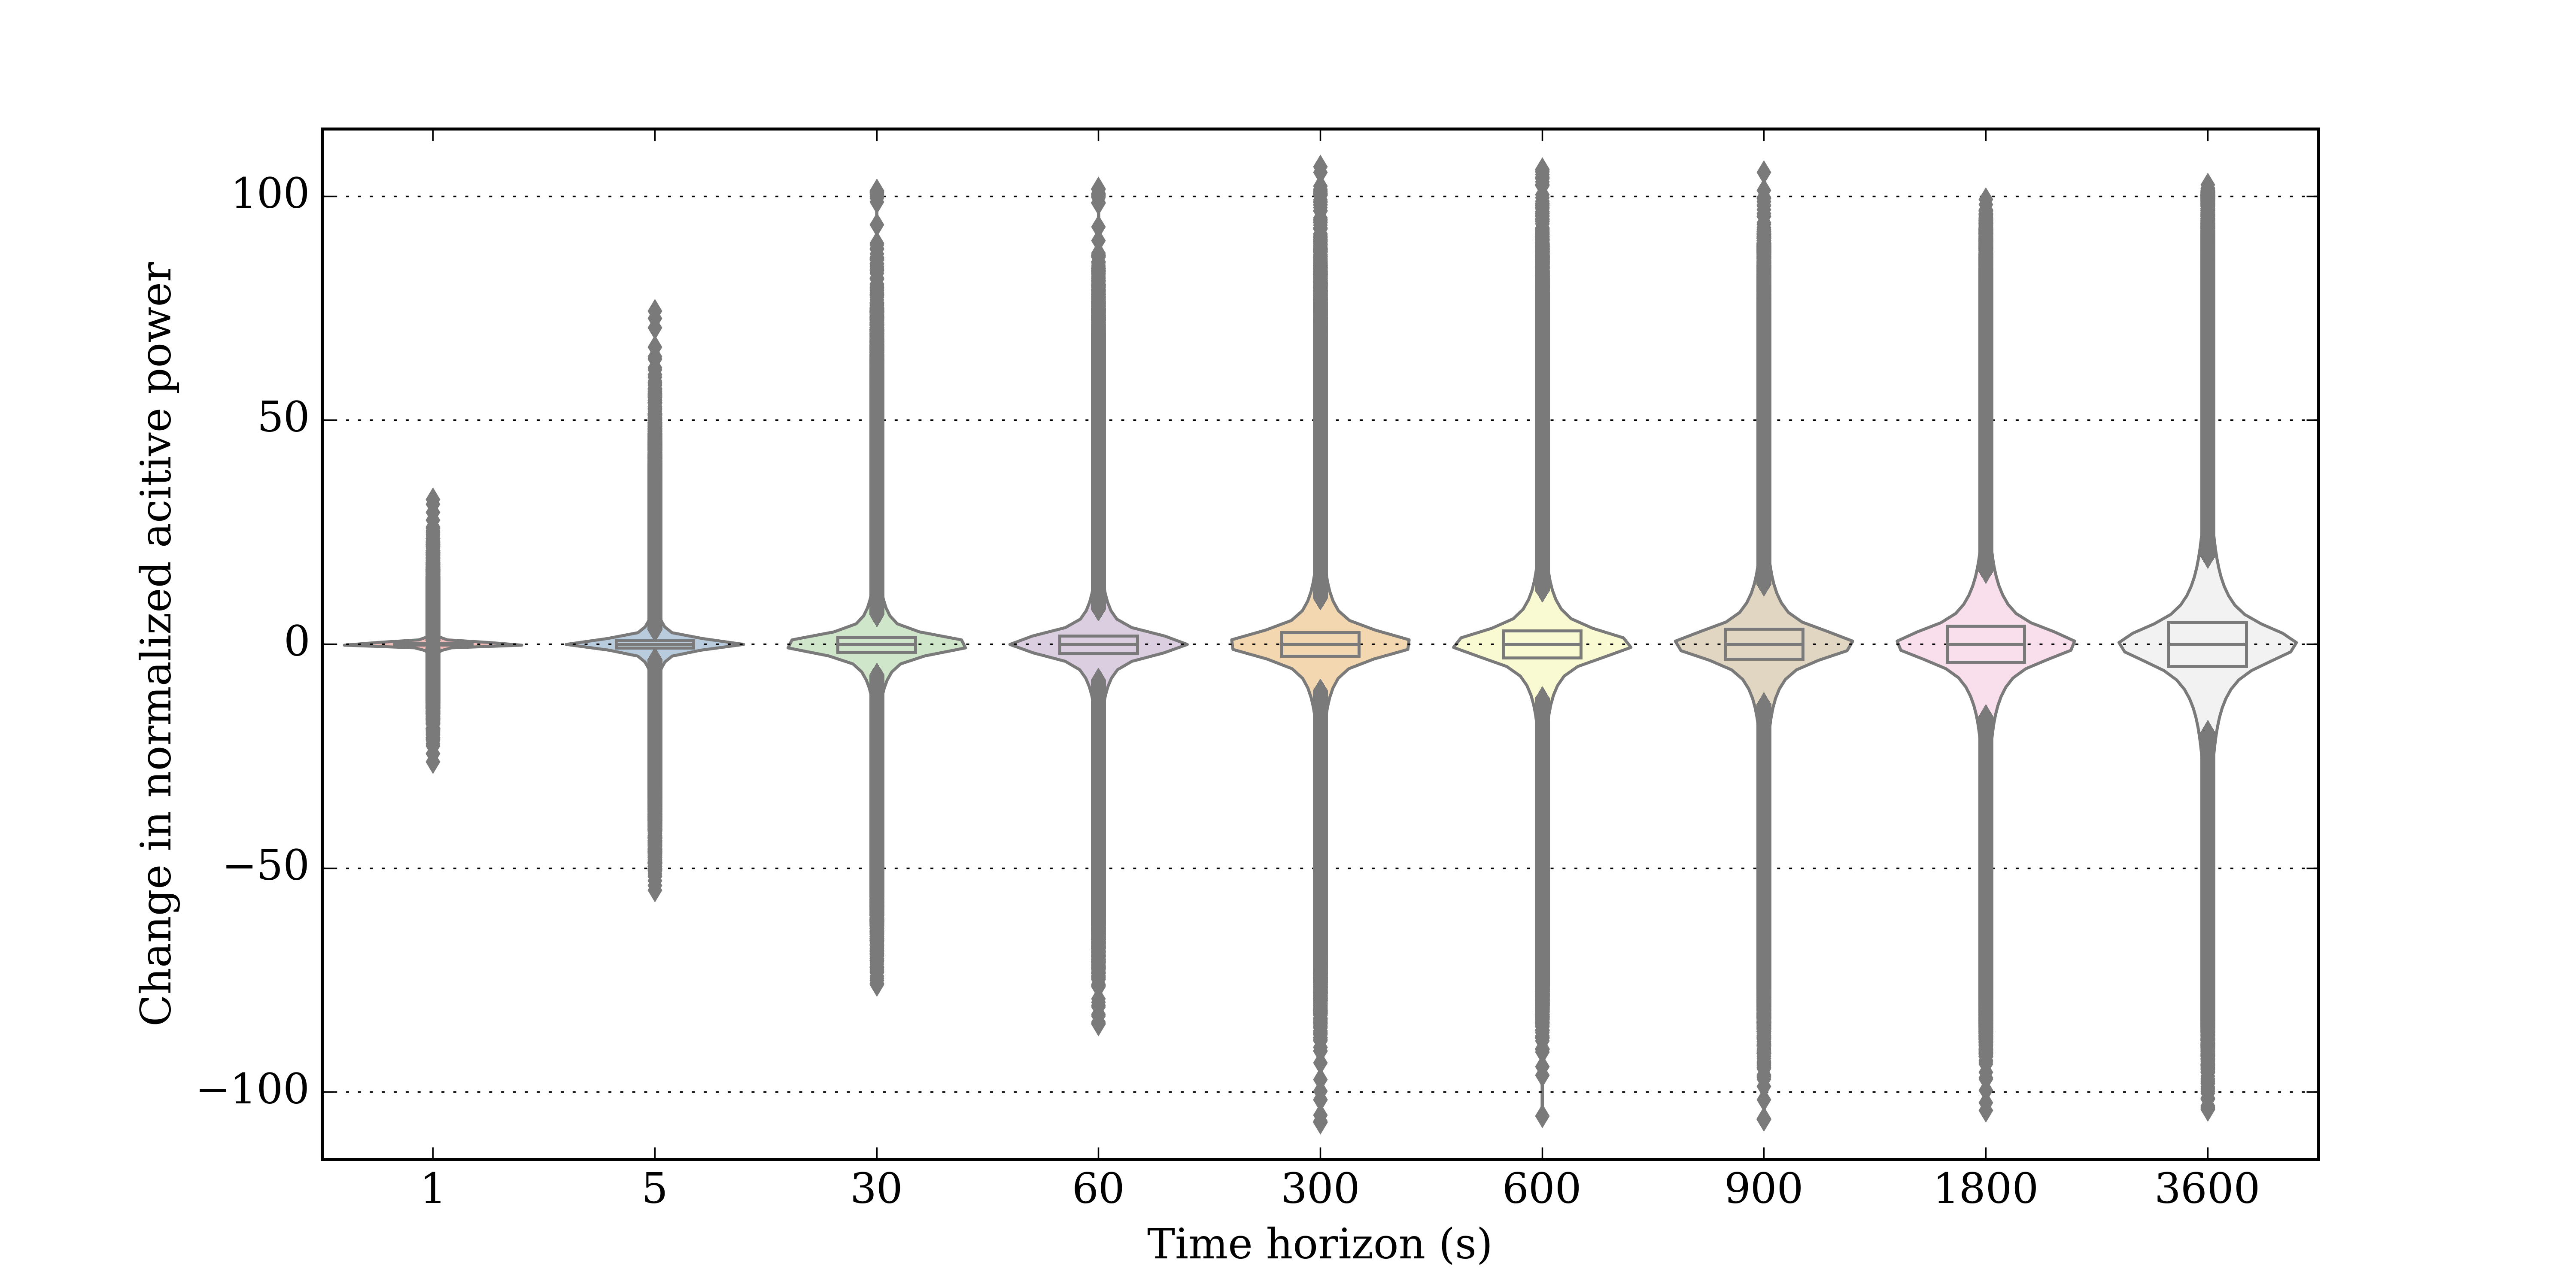
\includegraphics[width=1.0\textwidth]{graphics/intro/variability/act_pow_change_vioboxplot.png}
    \caption{Combined violin and boxplot of normalized active power changes by various time windows from DTU's V52 research wind turbine}
    \label{fig:act_pow_change_vioboxplot}
\end{figure}

\begin{table}
    \centering
    \caption{Table of statistics for V52 power output variability over selected time windows up to 1-hour}
    \resizebox{\columnwidth}{!}{%
\begin{tabular}{lrrrrrrrrr}
\toprule
{} &          1 s &          5 s &         30 s &         60 s &        300 s &        600 s &        900 s &       1800 s &       3600 s \\
\midrule
count &  2976599 &  2976595 &  2976570 &  2976540 &  2976300 &  2976000 &  2975700 &  2974800 &  2973000 \\
mean  &        0.000 &        0.000 &        0.000 &        0.000 &        0.002 &        0.003 &        0.004 &        0.008 &        0.009 \\
std   &        1.209 &        4.387 &        8.133 &        9.536 &       11.362 &       11.976 &       12.532 &       13.674 &       15.485 \\
min   &      -26.250 &      -54.907 &      -76.028 &      -84.816 &     -106.745 &     -105.303 &     -106.126 &     -104.044 &     -103.887 \\
25\%   &       -0.225 &       -0.888 &       -1.841 &       -2.103 &       -2.630 &       -3.075 &       -3.371 &       -4.049 &       -4.957 \\
50\%   &        0.000 &        0.000 &        0.000 &        0.000 &        0.000 &        0.000 &        0.000 &        0.000 &        0.000 \\
75\%   &        0.214 &        0.782 &        1.515 &        1.860 &        2.544 &        2.972 &        3.341 &        4.064 &        4.870 \\
max   &       32.326 &       74.414 &      101.242 &      101.663 &      106.567 &      106.013 &      105.350 &       99.266 &      102.539 \\
\bottomrule
\end{tabular}
}
    \label{tab:intro_v52_variability_statistics}
\end{table}

As expected, the variability grows with the length of the window. In all cases, the mean and median power output change is very close to zero and probability densities are symmetrical (normally distributed). On the very shortest timescales (1 and 5-seconds), the variations within the interquartile range (IQR) are small. However, from 30-seconds to 1-minute windows, the spread grows considerably. By the 5-minute case (300 s), the standard deviation approaches that of the longer timescales.
\\\\
This is further shown in Figure \ref{fig:norm_act_pow_error_dist}, where the distributions are stacked atop each other for comparison (note the logarithmic y-axis scaling). Tail bumps present for certain time windows near the peripheries indicate periods of automatic start up (right tail) when the cut-in wind speed is reached and shut down (left tail) when the cut-out wind speed is exceeded.

\begin{figure}[htbp]
    \centering
        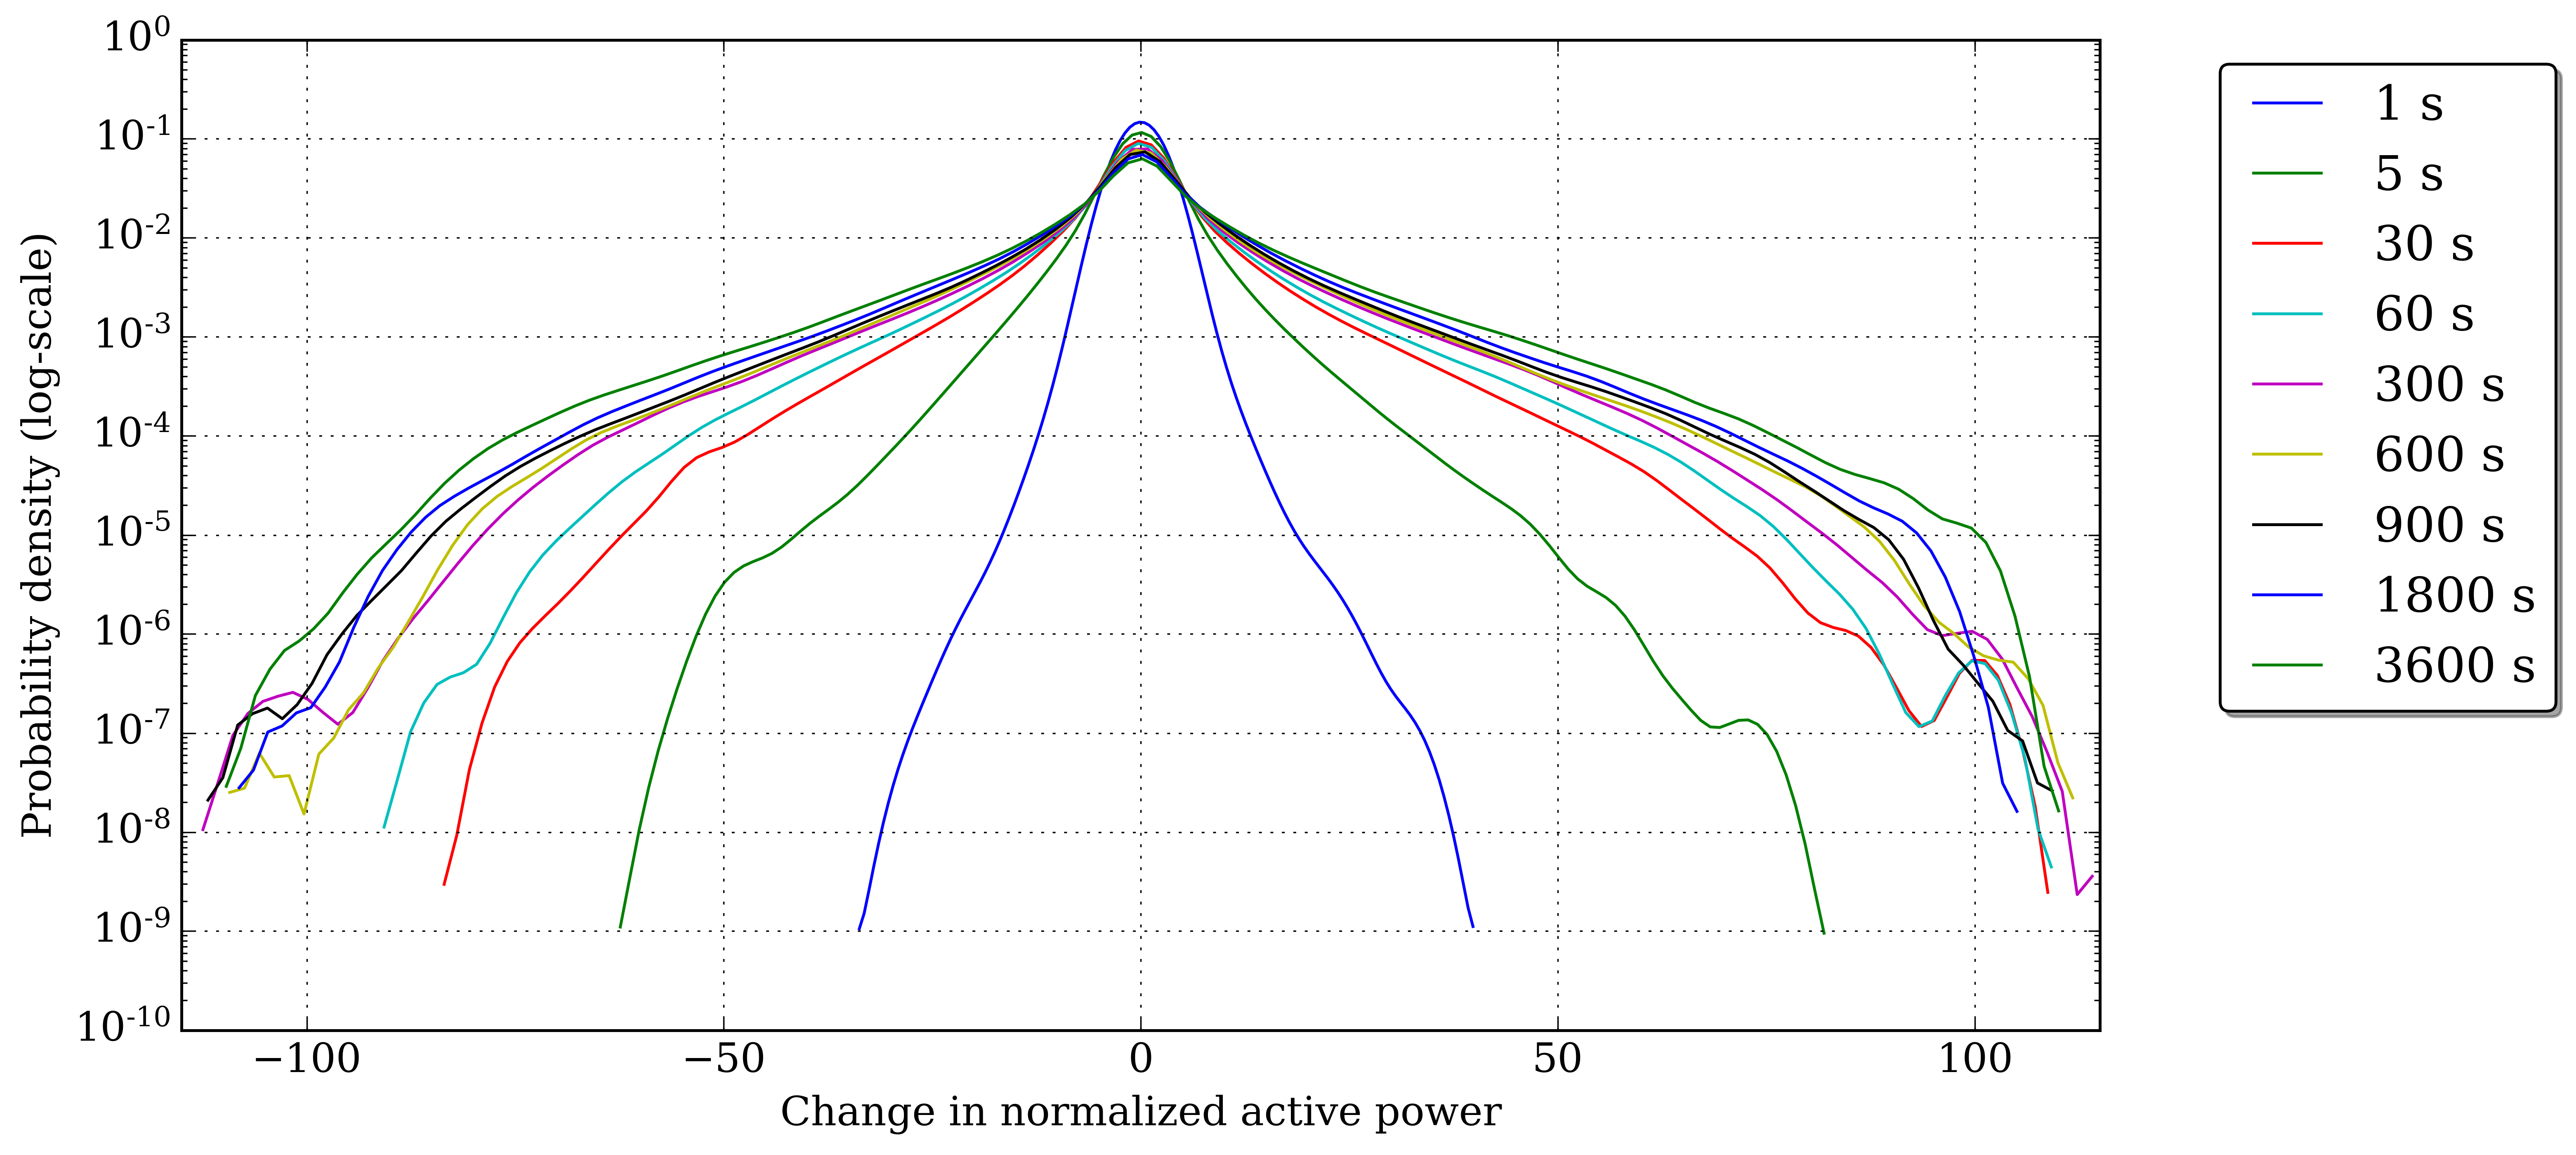
\includegraphics[width=1.0\textwidth]{graphics/intro/variability/norm_act_pow_error_dist.png}
    \caption{Distribution of changes in normalized active power over various time horizons from DTU's V52 research wind turbine}
    \label{fig:norm_act_pow_error_dist}
\end{figure}

This simplified investigation has considered a single wind turbine and not collective wind farm output or otherwise geographically distributed generation which will act to some degree as a smoothing filter. Having said that, the case study has demonstrated that minute-scale variability of wind power is not insignificant and attention should also be focused on this timescale alongside the more commonly focused periods (e.g. 1-hour).

%--------------------------------------------------------------------------------
\clearpage
\subsection{Forecasting for wind energy}
\label{sec:intro_forecasting}

Placeholder


%--------------------------------------------------------------------------------
\clearpage
\subsection{Power system and electricity markets}
\label{sec:intro_power_markets}

Placeholder




\begin{comment}
•	Errors in power forecast do not necessarily reflect impact. Overestimation and underproduction != underprediction and overproduction due to structure of balancing market.
•	The need for spinning reserves. Frequency control/response mode. Droop speed control. Spinning reserve is extremely expensive for utilities. 
•	https://en.wikipedia.org/wiki/Dynamic_demand_(electric_power)#The_need_for_spinning_reserve
•	Cost of imbalance not only money but also CO2
\end{comment}


%--------------------------------------------------------------------------------
\clearpage
\subsection{Wind turbine and wind farm control}
\label{sec:intro_control}

Placeholder


%--------------------------------------------------------------------------------
%--------------------------------------------------------------------------------
\clearpage
\section{Remote sensing}
\label{intro_remote_sensing}

%--------------------------------------------------------------------------------
\subsection{Principles}
\label{sec:intro_rs_principles}

Placeholder


%--------------------------------------------------------------------------------
\clearpage
\subsection{Lidar}
\label{sec:intro_lidar}

Placeholder


%--------------------------------------------------------------------------------
\clearpage
\subsection{Measurement techniques}
\label{sec:intro_meas_tech}

Placeholder


%--------------------------------------------------------------------------------
\clearpage
\subsection{Processing, filtering, and interpreting data}
\label{sec:intro_rs_data}

Placeholder

\clearpage